\documentclass{protokol}
\leftheader{Simulace průchodu částic hadronovým kalorimetrem}
\centerheader{}
\rightheader{Tomáš Derner}

\begin{document}

  \section*{Úkol}

    \begin{enumerate}
      \item Provést interaktivní simulace základních typů částic a zobrazit jednotlivé interakce,
      \item Kvantitativně porovnat energetické ztráty v kalorimetru pro různé druhy částic (elektron, mion, pion), 
      \item Prostudovat odezvu modelu kalorimetru a jeho energetické rozlišení
    \end{enumerate}

  \section*{Teorie}

    V tomto praktiku se zabýváme počítačovou simulací průchodu vysokoenergetických částic kalorimetrem. Model kalorimetru je implementován po vzoru experimentu ATLAS v CERNu. Modelovaný kalorimetr má délku \SI{150}{cm}, příčné rozměry $80 \times \SI{80}{cm}$ a obsahuje 75 střídavých vrstev železa a scintilátoru.

    Jedná se o simulaci destruktivního měření. Částice kalorimetru předá veškerou svoji energii, většinu ve vrstvách železa a část ve scintilátoru, kde je transformována ve světelné záblesky, které je možné sledovat a vyhodnocovat. Při průchodu kalorimetrem se částice rozpadají a vytvářejí tzv. spršku.

    Částice lze dle způsobu interakce s látkou rozdělit do skupin:
    \begin{enumerate}
      \item částice vytvářející čistě elektromagnetickou spršku ($e^-, e^+, \gamma, \pi^0$)
      \item částice produkující hadronovou spršku (vysokoenergetické hadrony kromě $\pi^0$)
      \item ionizující částice ($\mu$)
      \item neinteragující částice ($\nu$)
    \end{enumerate}

    V zájmu stručnosti byl popis jednotlivých způsobů interakce přenechán do sekce výsledků.

    Energetické rozlišení kalorimetru lze vyjádřit jako 
    \begin{equation}
      \frac{\sigma(E_{dep})}{E_{dep}} = \frac{a}{\sqrt{E_0}} + b,
    \end{equation}
    kde $E_0$ je původní energie částice a $a$ tzv. \textit{sampling term}.

    
  \section*{Výsledky}

    \subsection*{Úkol 1}

      Obrázky \ref{fig:elektron_20Gev} - \ref{fig:mu-} ukazují průlety částic kalorimetrem. Kvůli nesprávnému nastavení zobrazení interaktivní simulace byly výsledné snímky obrazovky barevně velice nevýrazné a nekontrastní. V mnoha případech také sprška zabírala jen malou část kalorimetru, při zobrazení celého snímku by zanikly detaily. Proto byly tyto snímky oříznuty a barevně vylepšeny softwarem pro digitální úpravu obrázků. 

      Jako první jsou zobrazeny elektromagnetické spršky elektronu (obr. \ref{fig:elektron_20Gev}), částice $\gamma$ (obr. \ref{fig:gamma_10GeV}) a $\pi^0$ (obr. \ref{fig:pi0_10GeV}). Elektromagnetické spršky vznikají opakovanou konverzí částice $\gamma$ na elektron-pozitronový pár, který následně brzdně září. Částice $\pi^0$ se s vysokou pravděpodobností (\SI{99}{\percent}) rychle rozpadá na $2 \gamma$ a ve zbytku případů na elektron pozitronový pár a $\gamma$. Na obrázku \ref{fig:pi0_10GeV} vlevo vstupují do kalorimetru dvě z těchto částic. Elektron je zobrazen modře, nenabité částice se nezobrazují.

    \begin{figure}[H]
      \centering
      \includegraphics[scale=1.9]{elektron_20Gev}
      \vspace{-10pt}
      \caption{Průlet elektronu s energií \SI{20}{GeV} kalorimetrem}
      \label{fig:elektron_20Gev}
    \end{figure}

    \vspace{-10pt}

    \begin{figure}[H]
      \centering
      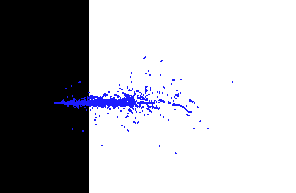
\includegraphics[scale=1.9]{gamma_10GeV}
      \vspace{-10pt}
      \caption{Průlet částice $\gamma$ s energií \SI{10}{GeV} kalorimetrem}
      \label{fig:gamma_10GeV}
    \end{figure} 

    \vspace{-10pt}

    \begin{figure}[H]
      \centering
      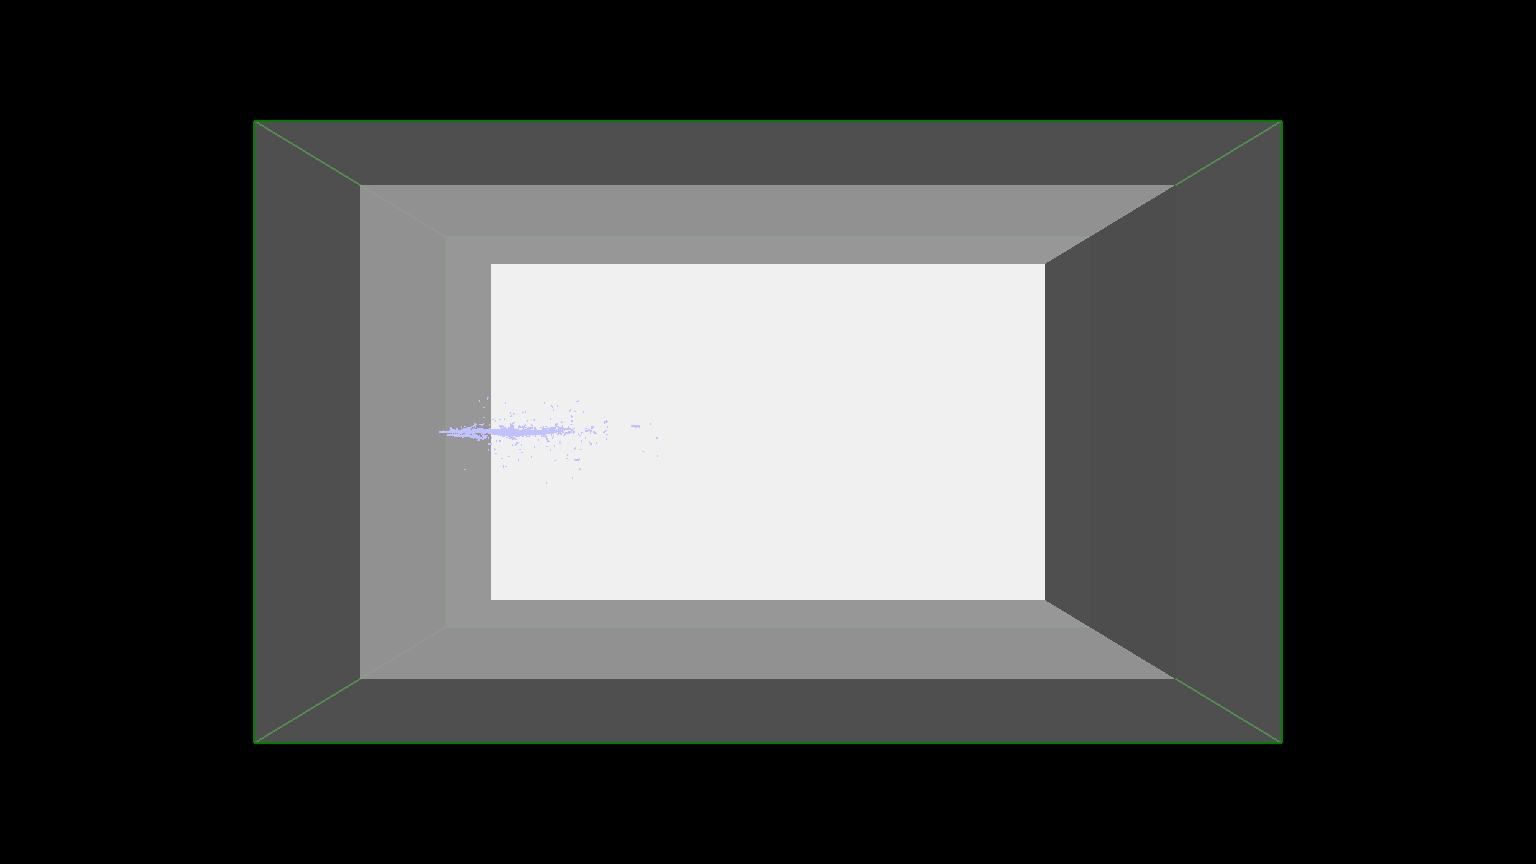
\includegraphics[scale=2.4]{pi0_10GeV}
      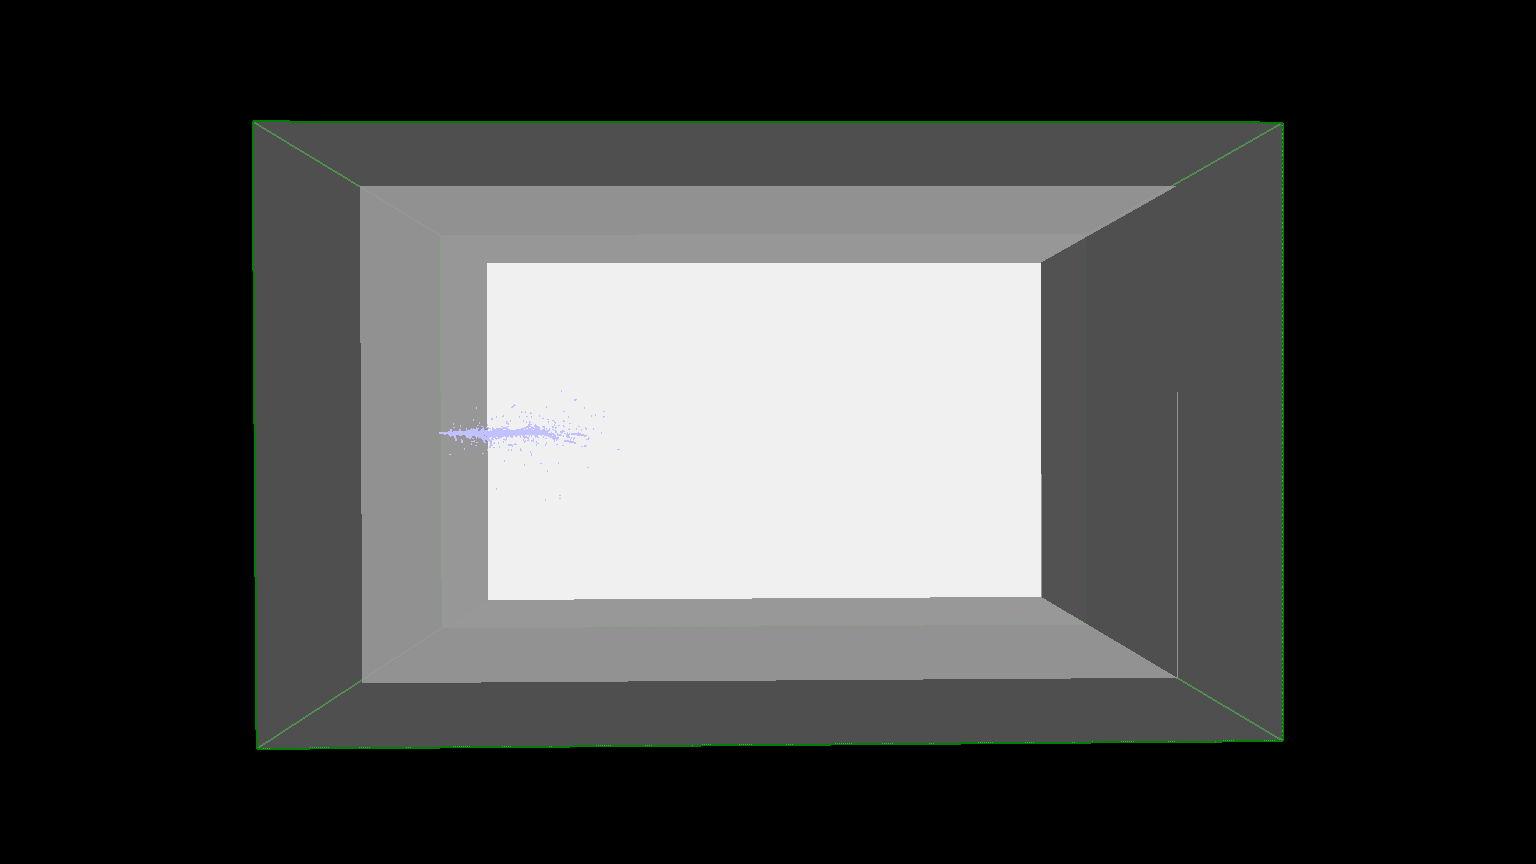
\includegraphics[scale=2.4]{pi0_2_10GeV}
      \vspace{-10pt}
      \caption{Průlet dvou částic $\pi^0$ s energií \SI{10}{GeV} kalorimetrem}
      \label{fig:pi0_10GeV}
    \end{figure}

    \vspace{-10pt}

    Obrázky \ref{fig:kaon+_10GeV} až \ref{fig:proton_10GeV} zachycují průlet částic produkujících hadronovou spršku. Ve všech případech jsou produktem další hadrony, především protony (světle modře) a částice $\pi$ (fialově). Interakce se liší převážně dobou života původní částice, viz obr. \ref{fig:kaon0_10GeV}, kde se částice $K_L^0$ (vlevo) šíří až za polovinu délky kalorimetru, kdežto $K_S^0$ se hned po dopadu na kalorimetr rozpadla. Všechny tyto interakce jsou dále doprovázeny sprškami elektromagnetickými. Kromě hadronů a elektronů nám zde také část energie unášejí neutrina, která jsou však vysoce nereaktivní a nezobrazují se.

    \begin{figure}[H]
      \centering
      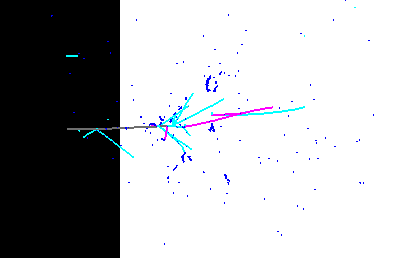
\includegraphics[scale=1.54]{kaon+_10GeV}
      \vspace{-10pt}
      \caption{Průlet částice $K^+$ s energií \SI{10}{GeV} kalorimetrem}
      \label{fig:kaon+_10GeV}
    \end{figure}

    \vspace{-10pt}

    \begin{figure}[H]
      \centering
      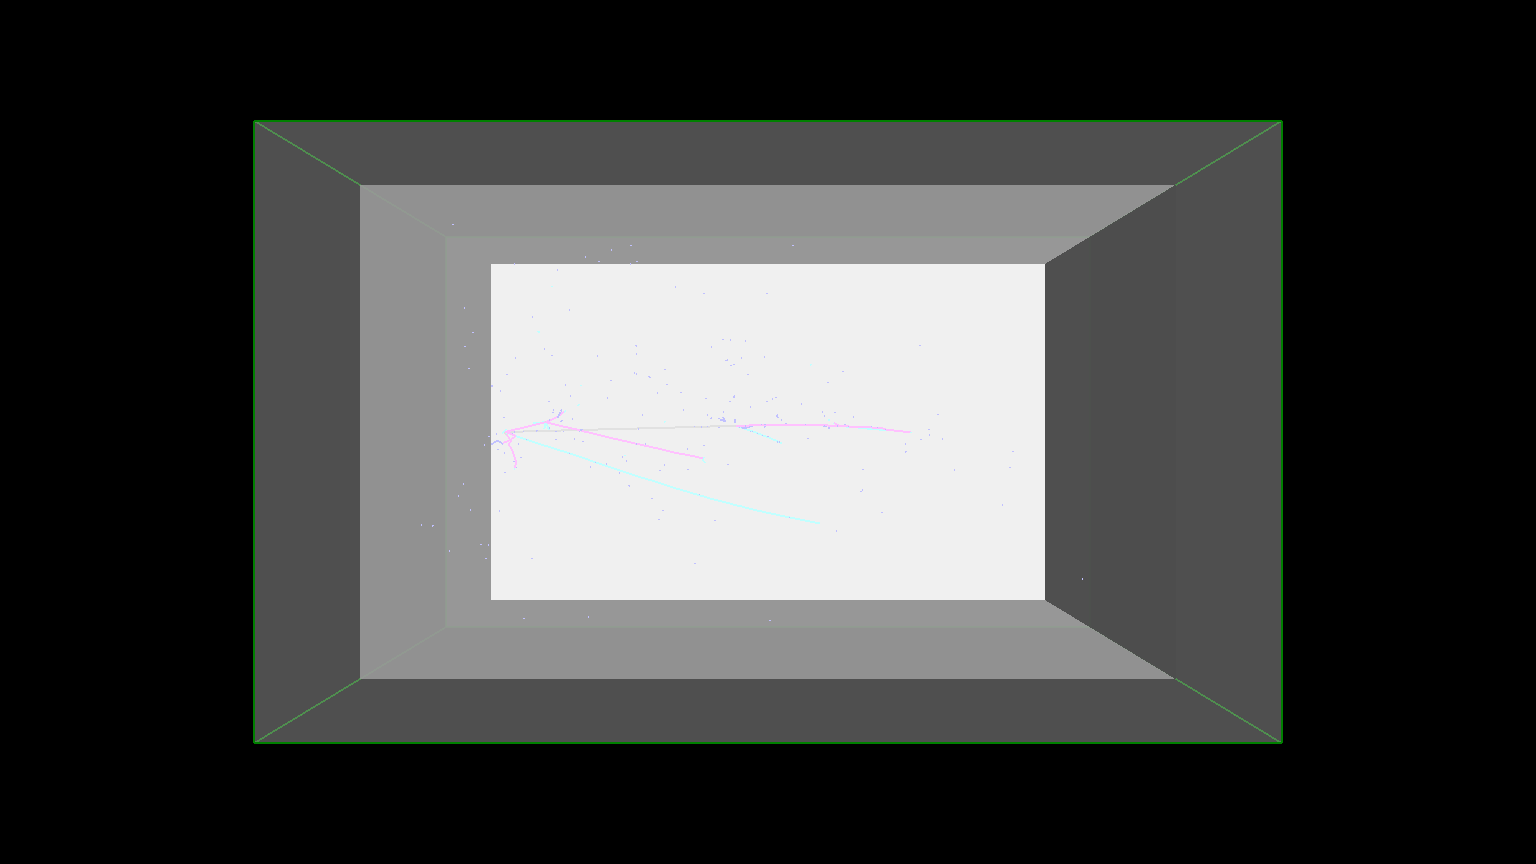
\includegraphics[scale=1.3]{kaon0L_10GeV}
      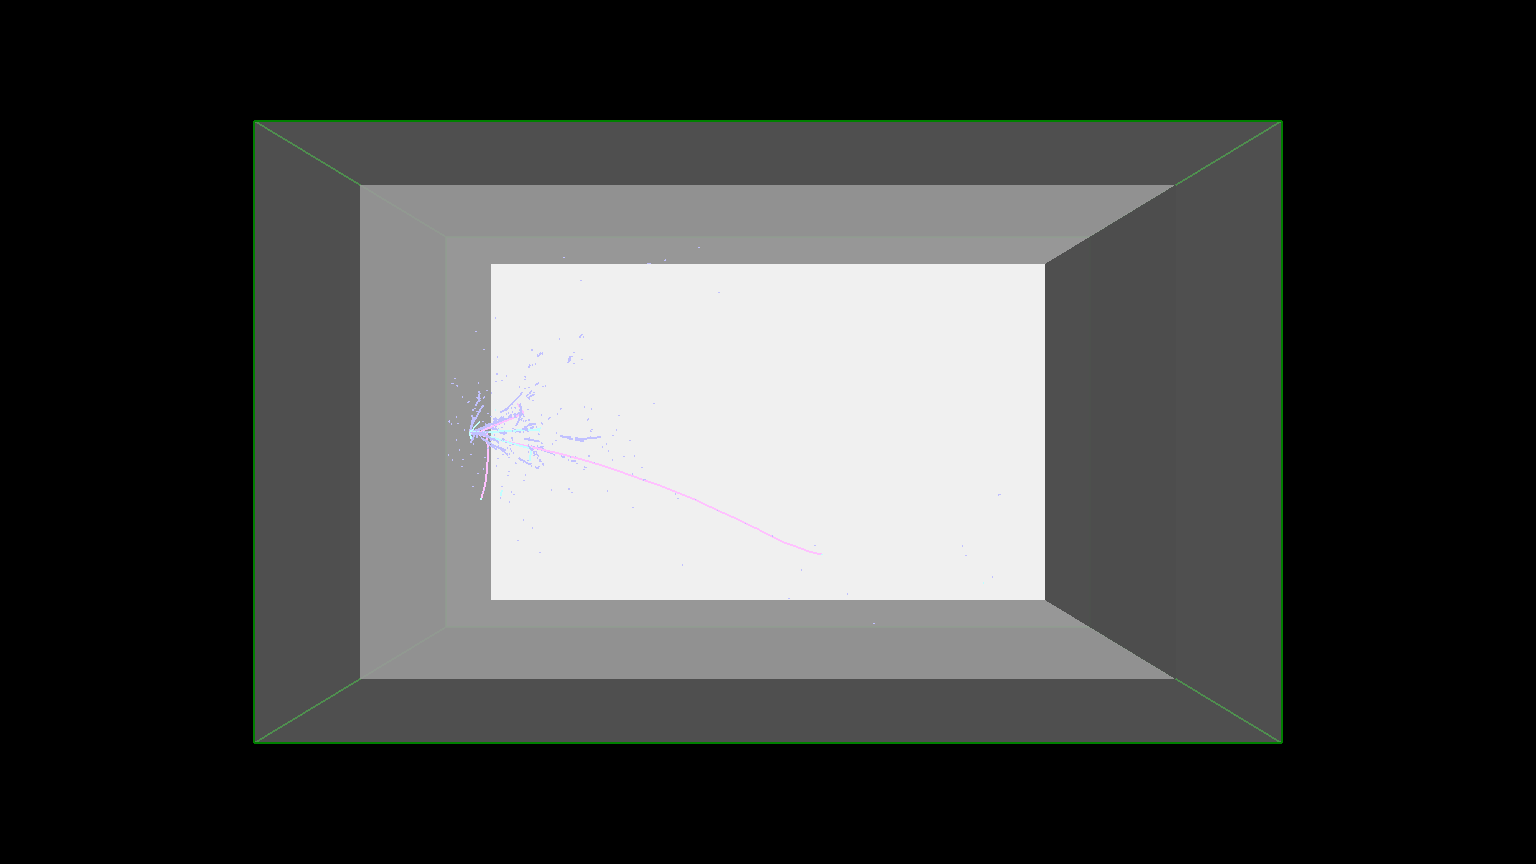
\includegraphics[scale=1.3]{kaon0S_10GeV}
      \vspace{-10pt}
      \caption{Průlet částic $K^0_L$ a $K^0_S$ s energií \SI{10}{GeV} kalorimetrem}
      \label{fig:kaon0_10GeV}
    \end{figure}

    \vspace{-10pt}

    \begin{figure}[H]
      \centering
      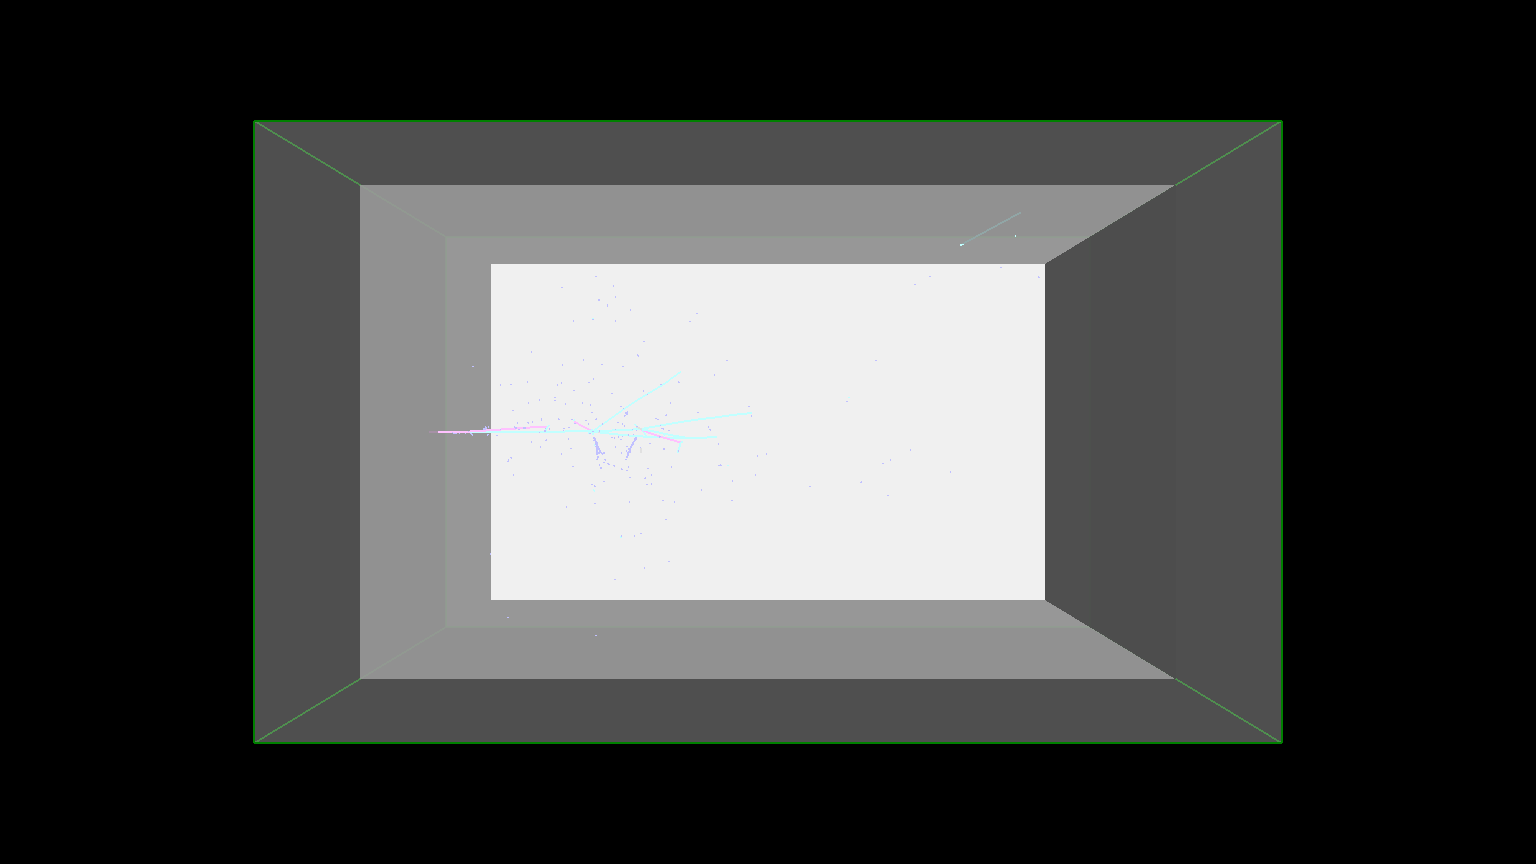
\includegraphics[scale=1.8]{lambda_10GeV}
      \vspace{-10pt}
      \caption{Průlet částice $\Lambda$ s energií \SI{10}{GeV} kalorimetrem}
      \label{fig:lambda_10GeV}
    \end{figure}

    \vspace{-10pt}

    \begin{figure}[H]
      \centering
      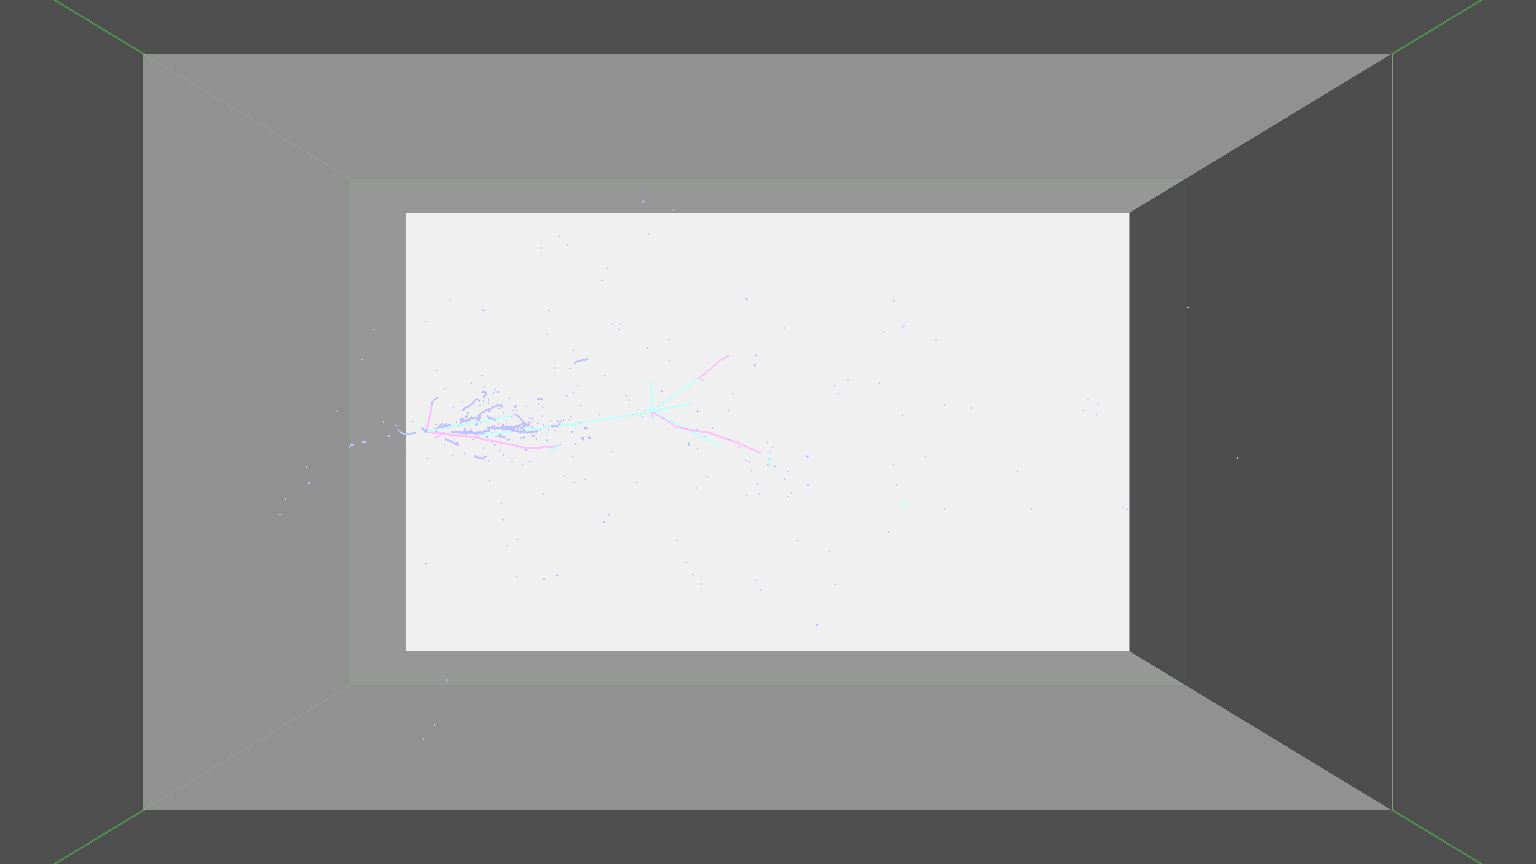
\includegraphics[scale=1.8]{neutron_10GeV}
      \vspace{-10pt}
      \caption{Průlet neutronu s energií \SI{10}{GeV} kalorimetrem}
      \label{fig:neutron_10GeV}
    \end{figure}

    \vspace{-10pt}

    \begin{figure}[H]
      \centering
      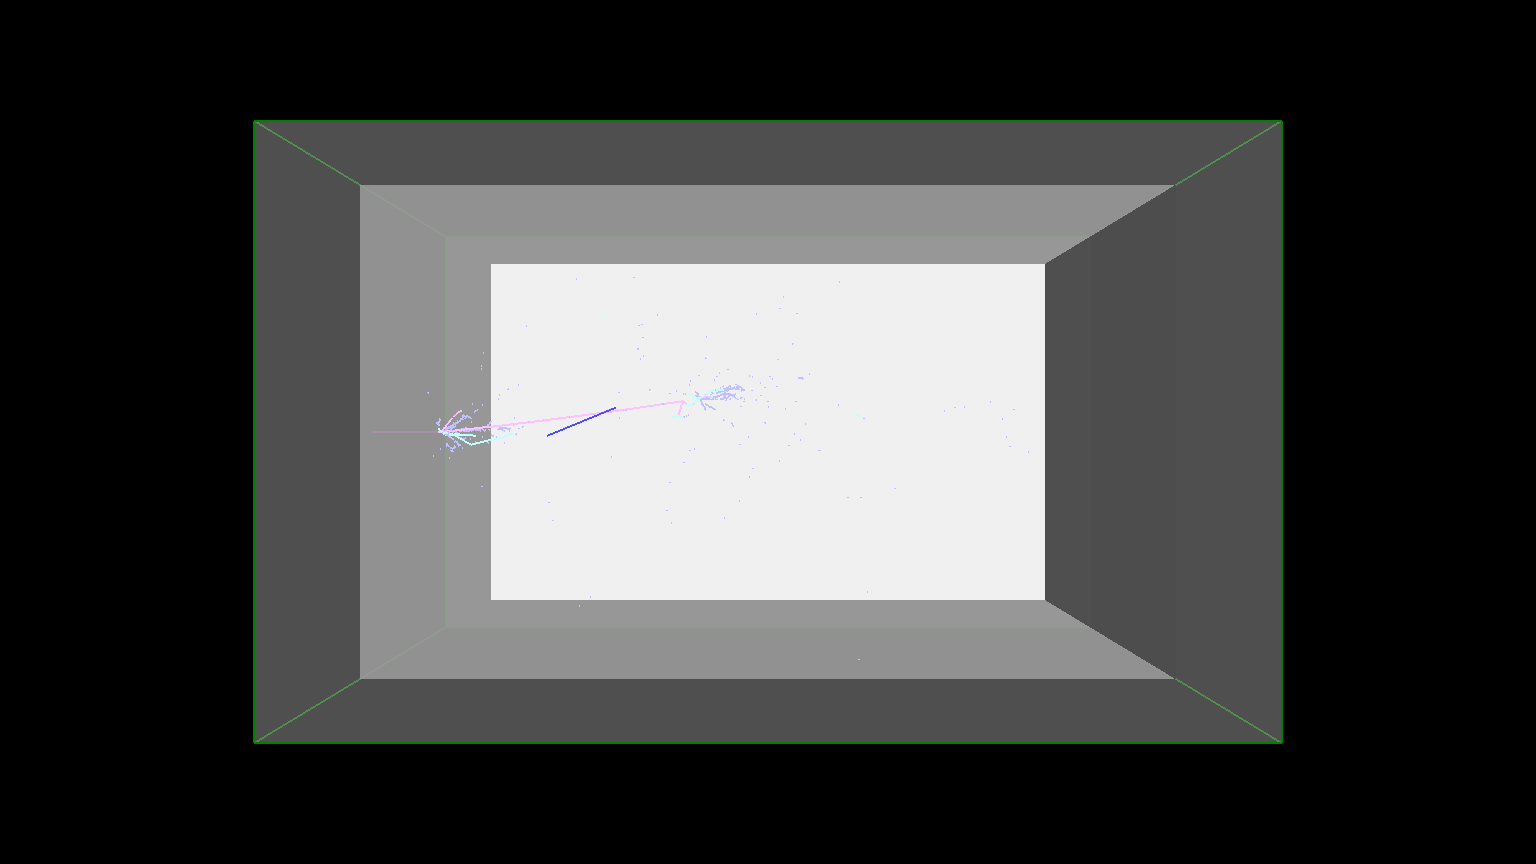
\includegraphics[scale=2.1]{pi-_10GeV}
      \vspace{-10pt}
      \caption{Průlet částice $\pi^-$ s energií \SI{10}{TeV} kalorimetrem}
      \label{fig:pi-_10GeV}
    \end{figure}

    \vspace{-10pt}

    \begin{figure}[H]
      \centering
      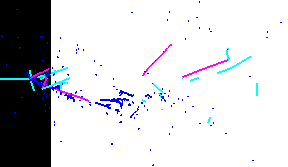
\includegraphics[scale=2]{proton_10GeV}
      \vspace{-10pt}
      \caption{Průlet protonu s energií \SI{10}{GeV} kalorimetrem} 
      \label{fig:proton_10GeV}
    \end{figure}

    \vspace{-10pt}

    Na obrázku \ref{fig:mu-} vidíme dva průlety částice $\mu^-$. Tato částice ztrácí jen minimum energie a kalorimetr vzápětí opouští. Tyto ztráty energie jsou způsobeny ionizací, z obrázku je patrné, že při vyšší energii je efekt ionizace větší.

    \begin{figure}[H]
      \centering
      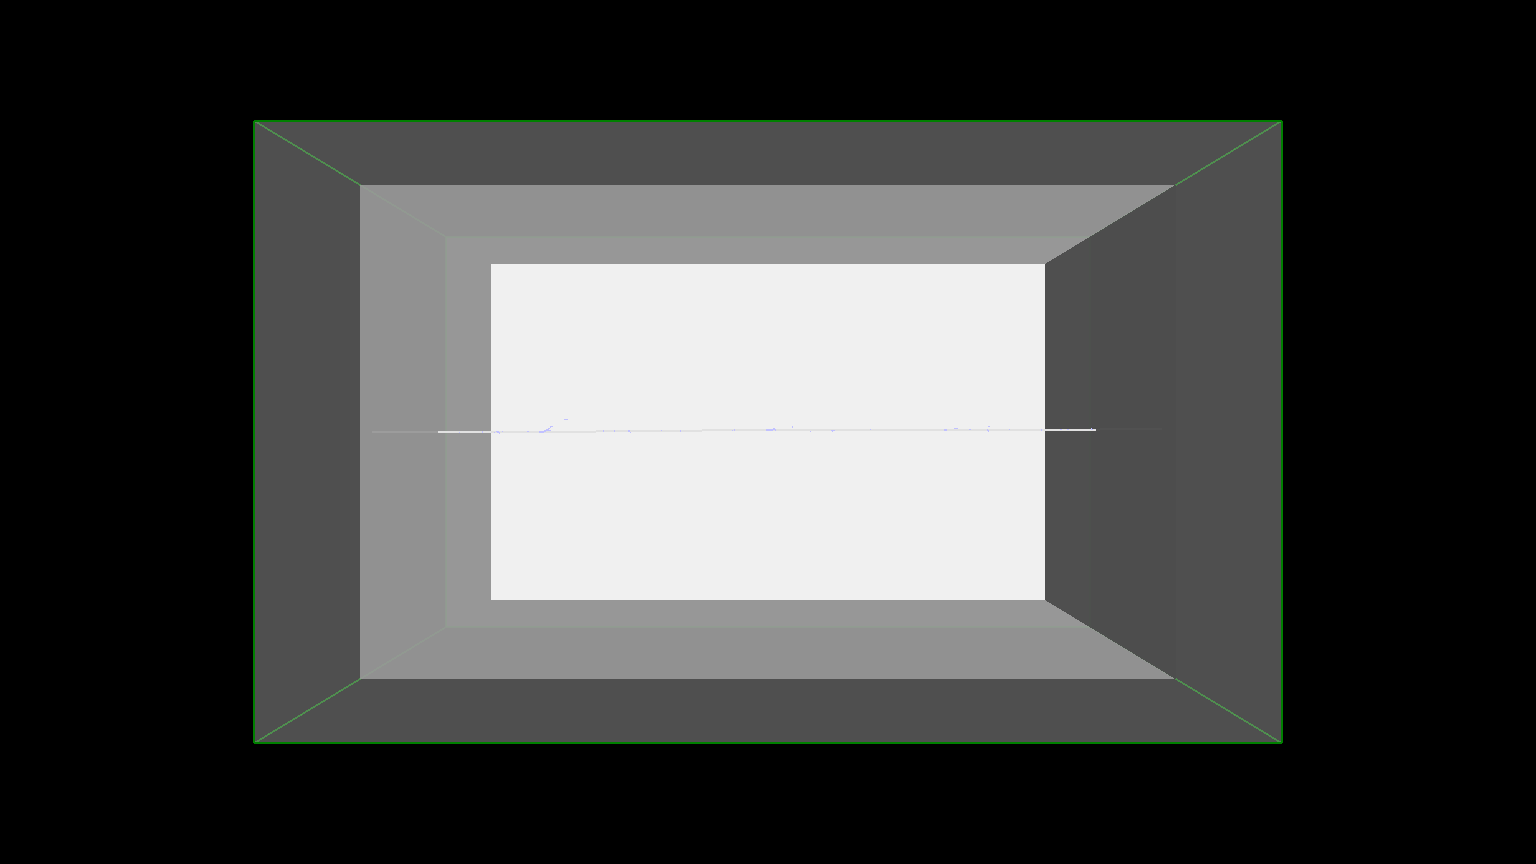
\includegraphics[scale=1.8]{mu-_10GeV}\\
      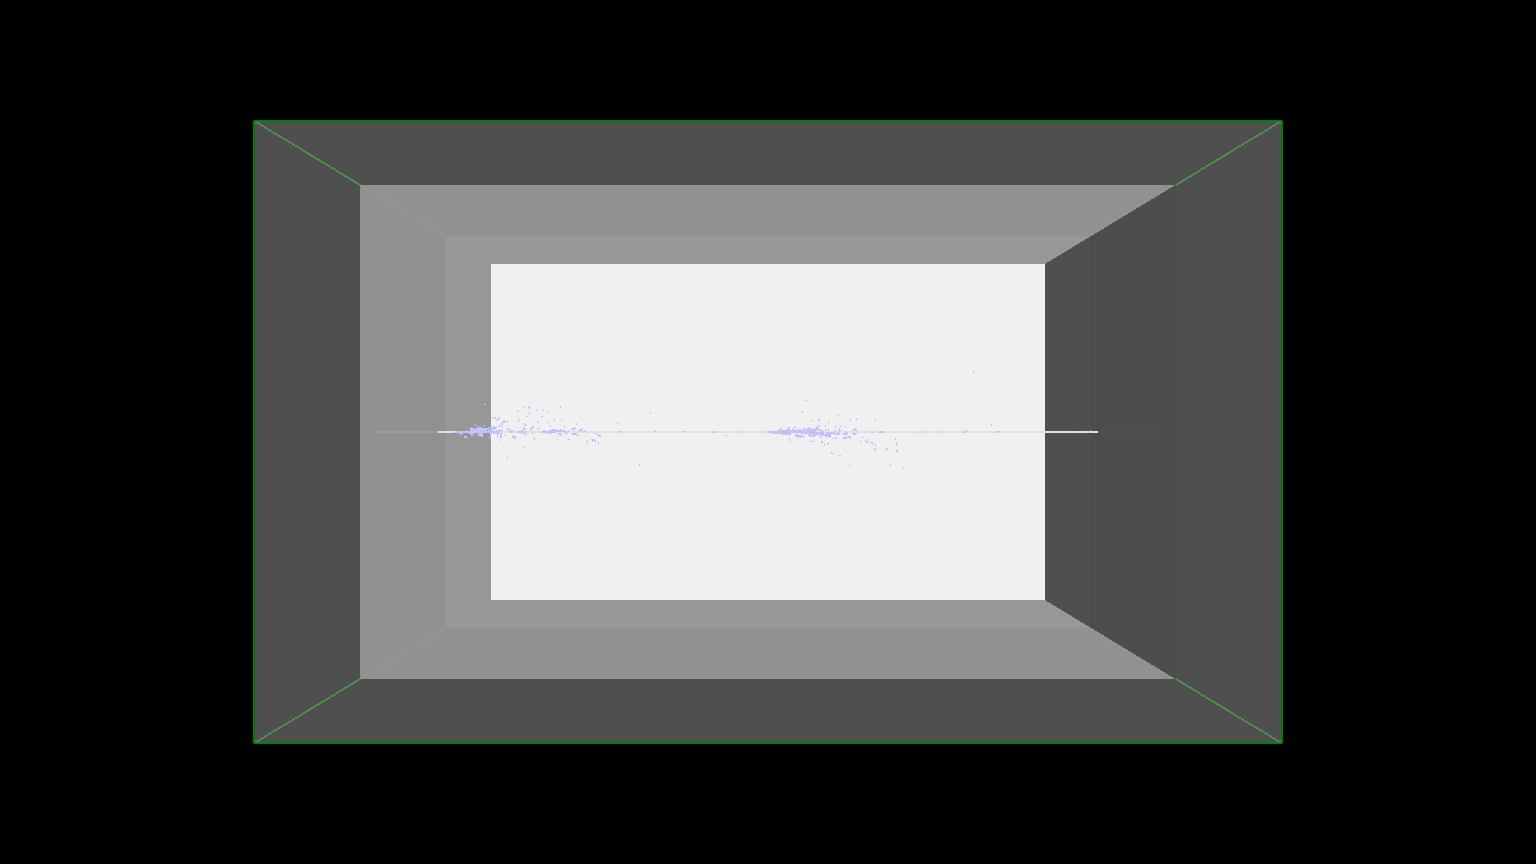
\includegraphics[scale=1.9]{mu-_2TeV}
      \vspace{-10pt}
      \caption{Průlet částice $\mu^-$ s energií \SI{10}{GeV} a \SI{2}{TeV} kalorimetrem}
      \label{fig:mu-}
    \end{figure}

  \subsection*{Úkol 2}

    V zadní části protokolu jsou přiloženy výstupy programu root z měření průchodu elektronu a částice $\mu$ a $\pi$ kalorimetrem. Všechny částice měly počáteční energii $\SI{17}{GeV}$.

    Z výsledků měření elektronu je zřejmé, že celá energie elektronu byla předána kalorimetru v jeho přední části, součet energie předané železu a scintilátoru se téměř rovná energii počáteční, úniky po stranách kalorimetru jsou zanedbatelné.

    Výsledky měření částice $\mu$ ukazují (společně s obrázkem \ref{fig:mu-}), že jen malá část energie ($\SI{12}{\percent}$) částice byla předána kalorimetru, a to rovnoměrně po celou dobu průletu. Většinu energie si částice odnesla s sebou po odchodu z kalorimetru. Úniky energie po stranách kalorimetru jsou opět zanedbatelné.

    Předávání energie částice $\pi$ probíhalo pozvolněji než v případě elektronu. Ze součtu energie předané železu a scintilátoru a z grafu ve spodní části přílohy je zřejmé, že nezanedbatelné množství energie uniklo po stranách kalorimetru.

  \subsection*{Úkol 3}

    Bylo provedeno 5 simulací průchodu elektronu s různou energií kalorimetrem. Byly zaznamenány hodnoty \textit{sampling term} $a_i$ pro ztráty energie v železe a $a_s$ pro ztráty energie v scintilátoru. Tyto hodnoty jsou uvedeny v tabulce.
     
    \begin{table}[H]
      \centering
      \setlength{\tabcolsep}{10pt}
      \begin{tabular}[t]{
  S[table-format=1.0]
  S[table-format=2.1]
} \toprule
{$d$}  & {$I$}  \\
{[cm]} & {[nA]} \\ \midrule
     2 & 6.9 \\
     3 & 10.5 \\
     4 & 12.5 \\
     5 & 12.5 \\
     6 & 12.5 \\ \bottomrule
\end{tabular}
      \caption{Tabulka hodnot pro úkol 3}
      \label{tab:u3}
    \end{table}

    Jak lze vidět z grafů na obrázku \ref{fig:u3}, není závislost $a$ na $\sqrt{E_0}$ ani přibližně lineární, bylo proto od určení energetického rozlišení kalorimetru upuštěno.

    \begin{figure}[H]
      \centering
      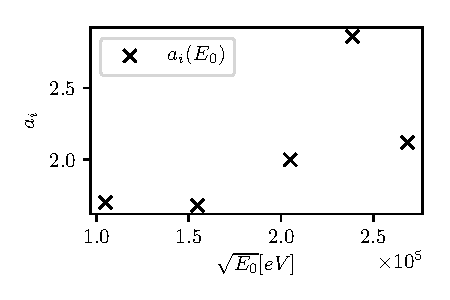
\includegraphics[]{u3_i2}
      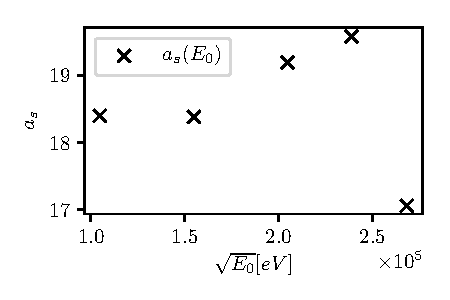
\includegraphics[]{u3_s2}
      \caption{Závislost $a_i$ a $a_s$ na odmocnině počáteční energie $E_0$}
      \label{fig:u3}
    \end{figure}

    % \begin{figure}[H]
    %   \centering
    %   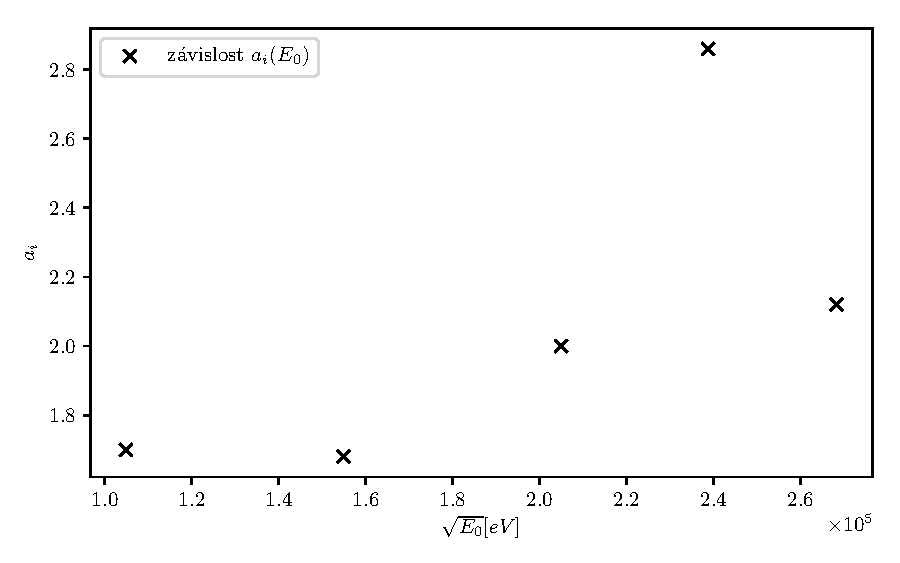
\includegraphics[]{u3_i}
    %   \caption{Závislost $a_i$ na odmocnině počáteční energie $E_0$}
    %   \label{fig:u3_i}
    % \end{figure}

    % \begin{figure}[H]
    %   \centering
    %   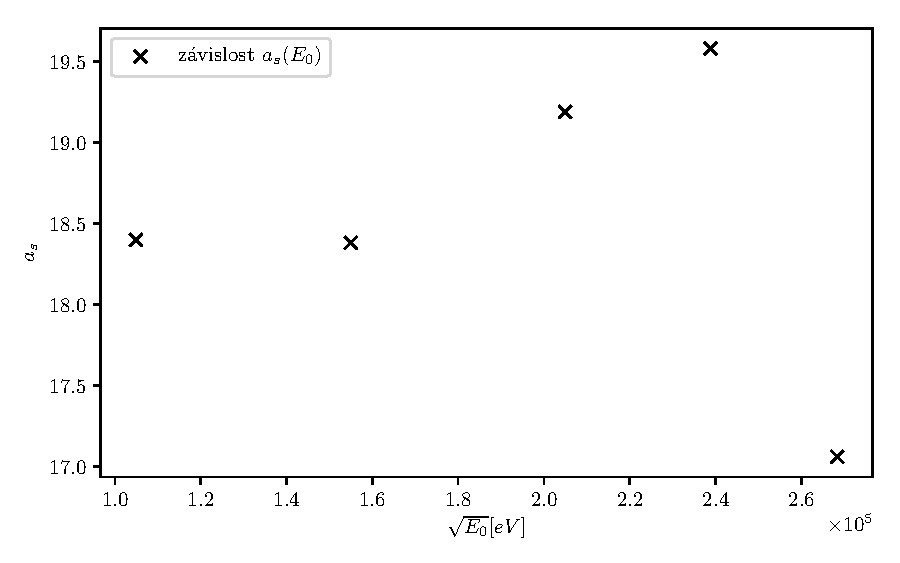
\includegraphics[]{u3_s}
    %   \caption{Závislost $a_s$ na odmocnině počáteční energie $E_0$}
    %   \label{fig:u3_s}
    % \end{figure}

  \section*{Diskuse}
    
    Jelikož toto praktikum bylo teoretičtějšího rázu a neproběhlo žádné skutečné měření, proběhla diskuse již v rámci shrnutí výsledků výše.

  \section*{Závěr}

    Byly provedeny a popsány interaktivní simulace průchodu částic kalorimetrem.

    Byly popsány průběhy energetických ztrát v kalorimetru pro elektron a částice $\mu$ a $\pi$.

    Z důvodu nelinearity závislosti $a(\sqrt(E_0))$ nebylo možné určit energetické rozlišení kalorimetru.


  \begin{thebibliography}{}
 
    \bibitem{pokyny}
    Pokyny k měření ``Simulace průchodu vysokoenergetických částic
    kalorimetrem'', dostupné z\\ \url{https://physics.mff.cuni.cz/vyuka/zfp/_media/zadani/texty/txt_406.pdf}, 10.\,10.\,2018
   
  \end{thebibliography}

\end{document} 